\documentclass{article}
\usepackage{listings}
\usepackage{graphicx}
\usepackage[slovene]{babel}
\usepackage{color}
\usepackage{amsmath}
\usepackage[usenames,dvipsnames]{xcolor}
\usepackage[hidelinks]{hyperref}
\usepackage{subcaption}
\usepackage{float}
\usepackage{rotating} 
\usepackage{hyperref}
\usepackage{caption}
\graphicspath{{./images/}}

\setlength{\parindent}{0pt}

\newcommand{\MAD}{\mathrm{MAD}}


\begin{document}

\title{Matematično-fizikalni praktikum \\[3mm] \large Naloga 6}
\author{Luka Papež}
\date{23.\ november 2024}

\begin{center}
    
\includegraphics[width=8cm]{logo-fmf.png}
\end{center}

{
    \let\newpage\relax
    \maketitle
}

\maketitle
\newpage
\section{Naloga}

{\it Naloga\/}: preizkusi preprosto Eulerjevo metodo ter nato še čim več 
naprednejših metod( Midpoint, Runge-Kutto 4. reda, Adams-Bashfort-Moultonov prediktor-korektor \ldots ) na primeru
z začetnima temperaturama $y(0)=21$ ali $y(0)=-15$,
zunanjo temperaturo $y_\mathrm{zun}=-5$ in parametrom $k=0.1$.
Kako velik (ali majhen) korak $h$ je potreben?
Izberi metodo (in korak) za izračun družine rešitev
pri različnih vrednostih parametra $k$.
\\
{\it Dodatna naloga\/:} temperatura prostora se lahko še
dodatno spreminja zaradi denimo sončevega segrevanja
skozi okna, s $24$-urno periodo in nekim faznim zamikom $\delta$,
kar opišemo z dva- ali triparametrično enačbo
\begin{equation}
\Dd{T}{t} = - k \left( T-T_\mathrm{zun} \right)
+ A\sin\left( {2\pi\over 24}(t-\delta) \right) \>.
\label{cooling2}
\end{equation}
Poišči še družino rešitev te enačbe pri
$k=0.1$ in $\delta=10$!  Začni z $A=1$, kasneje spreminjaj tudi
to vrednost.  V premislek: kakšno metodo bi uporabil, če bi posebej
natančno želel določiti maksimalne temperature in trenutke,
ko nastopijo?
\section{Uvod}
Za opis najpreprostejših fizikalnih procesov uporabljamo
navadne diferencialne enačbe, ki povezujejo vrednosti
spremenljivk sistema z njihovimi časovnimi
spremembami. Tak primer je na primer enačba za časovno
odvisnost temperature v stanovanju, ki je obdano s stenami
z neko toplotno prevodnostjo in določeno zunanjo temperaturo.
V najpreprostejšem primeru ima enačba obliko
\begin{equation}
\Dd{T}{t} = - k \left( T-T_\mathrm{zun} \right)
\label{cooling}
\end{equation}
z analitično rešitvijo
\begin{equation*}
T(t) = T_\mathrm{zun} + \mathrm{e}^{-kt} \left( T(0) - T_\mathrm{zun} \right) \>.
\end{equation*}
Enačbam, ki opisujejo razvoj spremenljivk sistema $y$ po času ali drugi
neodvisni spremenljivki $x$, pravimo {\sl enačbe hoda\/}.  Pri tej
nalogi bomo proučili uporabnost različnih numeričnih metod
za reševanje enačbe hoda oblike $\ddd y/\ddd x = f(x, y)$,
kot na primer~(\ref{cooling}).   Najbolj groba
prva inačica, tako imenovana osnovna Eulerjeva metoda,
je le prepisana aproksimacija za prvi odvod
$y' \approx (y(x+h) - y(x)) / h$, torej
\begin{equation}
y(x+h) = y(x) + h\,\left.\Dd{y}{x}\right|_x \>.
\label{euler}
\end{equation}
Diferencialno enačbo smo prepisali
v diferenčno: sistem
spremljamo v ekvidistantnih korakih dolžine $h$. Metoda je
večinoma stabilna, le groba: za večjo natančnost moramo
ustrezno zmanjšati korak.   Za red boljša (${\cal O}\,(h^3 )$ , t.j. lokalna natančnost drugega reda)
je simetrizirana Eulerjeva (ali sredinska) formula, ki sledi
iz simetriziranega približka za prvi odvod,
$y' \approx (y(x+h) - y(x-h)) / 2h$.  Računamo po shemi
\begin{equation}
y(x+h) = y(x-h) + 2h\,\left.\Dd{y}{x}\right|_x \>,
\label{seuler}
\end{equation}
ki pa je praviloma nestabilna.  Želeli bi si
pravzaprav nekaj takega
\begin{equation}
y(x+h) = y(x) + {h\over 2}\,\left[\left.\Dd{y}{x}\right|_x
+ \left.\Dd{y}{x}\right|_{x+h} \right] \>,
\label{impeuler}
\end{equation}
le da to pot ne poznamo odvoda v končni točki intervala
(shema je implicitna). Pomagamo si lahko z iteracijo.
Zapi\v simo odvod kot:
$$ \left.{dy \over dx}\right|_x = f(x,y) $$ ter $$ x_{n+1} = x_n + h,
~~~ y_n = y(x_n)$$
Heunova metoda (${\cal O}\,(h^3 )$ lokalno) je pribli\v zek idealne formule z:
\begin{eqnarray}
\hat{y}_{n+1} & =  & y_n +  h \cdot f(x_n,y_n) \\
y_{n+1} & = & y_n + \frac{h}{2} \left[ f(x_n,y_n) + f(x_{n+1},\hat{y}_{n+1})\right]
\end{eqnarray}
Izvedenka tega je nato Midpoint metoda  (tudi ${\cal O}\,(h^3 )$ lokalno):
\begin{eqnarray}
k_1 & = & f(x_n,y_n) \\
k_2 & = & f(x_n+{1 \over 2}h,y_n+{1 \over 2}\, h\,k_1) \\
y_{n+1} & = & y_n + h\,k_2
\end{eqnarray}
Le-to lahko potem izbolj\v samo kot modificirano Midpoint metodo
itd\ldots

V praksi zahtevamo natančnost in numerično učinkovitost,
ki sta neprimerno boljši kot pri opisanih preprostih metodah.
Uporabimo metode, zasnovane na algoritmih prediktor-korektor,
metode višjih redov iz družine Runge-Kutta (z adaptivnimi koraki), ali ekstrapolacijske metode.
Brez dvoma ena najbolj priljubljenih je metoda RK4,
\begin{align}
k_1 & =
  f\left(x,\,{y}(x)\right) \> {,}\nonumber\\
k_2 & =
  f\left(x+{\textstyle{1\over 2}}h,\,
       {y}(x)+{\textstyle{h\over 2}}k_1\right) \> {,}\nonumber\\
k_3 & =
  f\left(x+{\textstyle{1\over 2}}h,\,
       {y}(x)+{\textstyle{h\over 2}}k_2\right) \> {,}\label{eq:rk4}\\
k_4 & =  f\left(x+h,\,{y}(x)+hk_3\right) \> {,}\nonumber\\
{y}(x+h) & =  {y}(x)
  + {\tfrac{h}{6}}\,\left(k_1 + 2k_2 + 2k_3 + k_4\right) + {\cal O}(h^5)
  \nonumber\> {.}
\end{align}
\section{Rešitev}
\subsection{Eulerjeva metoda}
Zastavljena naloga nam poda izziv spremljanja spremembe temperature glede na dani odvod po času. To je v drug besedah integriranje. Kot v uvod v reševanje si najprej poglejmo najpreprostejšo Eulerjevo metodo numeričnega integriranja. Kot je podano v navodilu smo v odvodu $\frac{dT}{dt} = -k(T -T_{zun})$ določili vrednosti konstant $k=0.1$, $T_{zun}=-5$ za primera pa sta nam bili določeni temperaturi $T_0 = -15$ in $T_0=21$.

\begin{figure}[H]
    \centering
    \begin{subfigure}{0.49\textwidth}
        \centering
        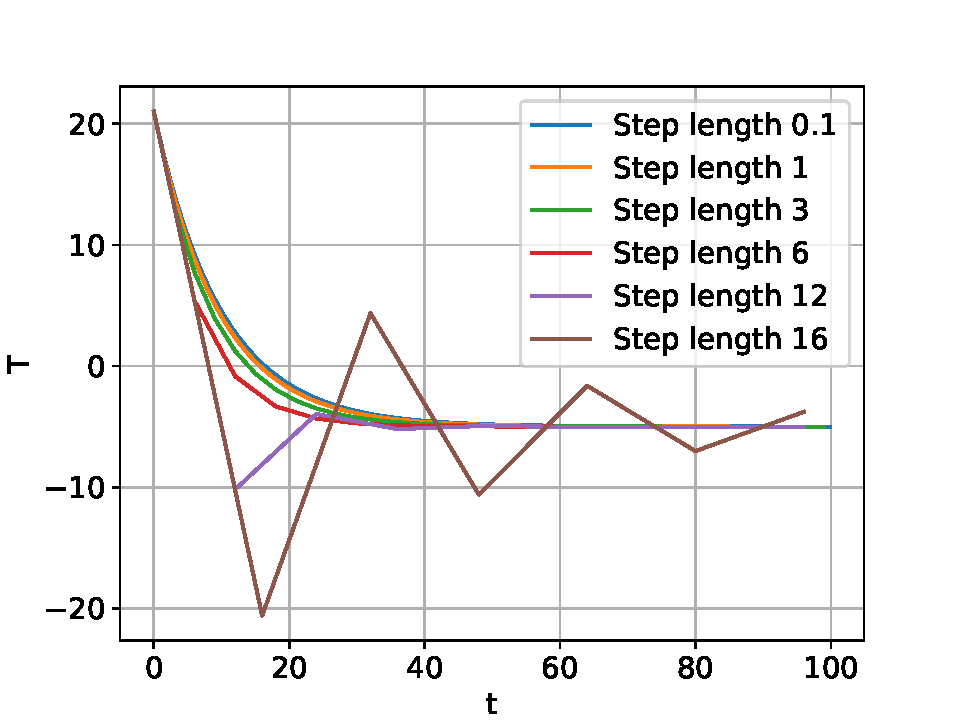
\includegraphics[width=\linewidth]{euler21.pdf}
        \caption{Ob začetni temperaturi $T=21$}
        \label{fig:image1}
    \end{subfigure}
    \hfill
    \begin{subfigure}{0.49\textwidth}
        \centering
        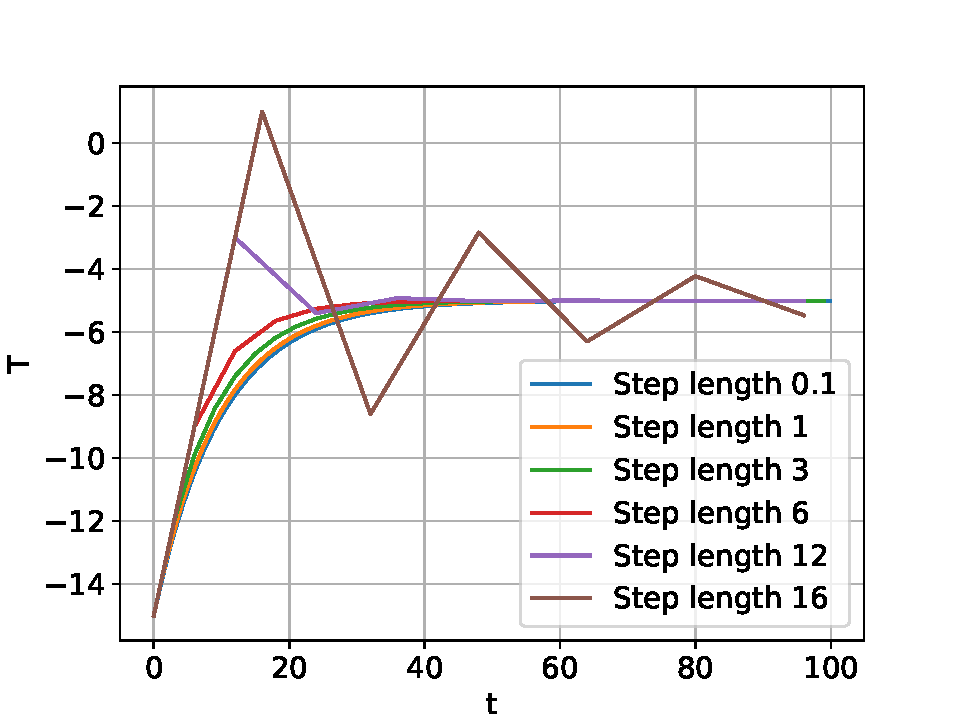
\includegraphics[width=\linewidth]{euler-15.pdf}
        \caption{Ob začetni temperaturi $T=-15$}
        \label{fig:image2}
    \end{subfigure}
	\caption{Spreminjanje temperature skozi čas pri različni dolžini korakov}
\end{figure}
Za računanje Eulerjeve metode sem najprej napisal svojo funkcijo nato pa sem opazil, da so nam podane že vse metode tudi na spletni učilnici. Nato je sledilo rahlo presenečenje, saj je podana funkcija vrnila drugačen slabši rezultat od moje. Po nadaljnjem raziskovanju sem opazil, da je v podani funkciji tip v numpy tabeli vrednosti odvisen od tipa podane začetne vrednosti. To napako sem preprosto odpravil tako, da sem spremenil ustvarjanje tabele na uporabo numpyeve funkcije `zeros`. Po popravku podane kode sem dobil prave vrednosti. Ta izkušnja okrepi nauk, da je vedno potrebno preveriti delovanje kode preden jo uporabiš. 
\newpage
\subsection{Izbira metode}
V tem podpoglavju je namen preizkusiti natančnost in časovno zahtevnost čim večih metod za poznejše računanje družin rešitev.


\begin{figure}[H]
    \centering
    \begin{subfigure}{0.49\textwidth}
        \centering
        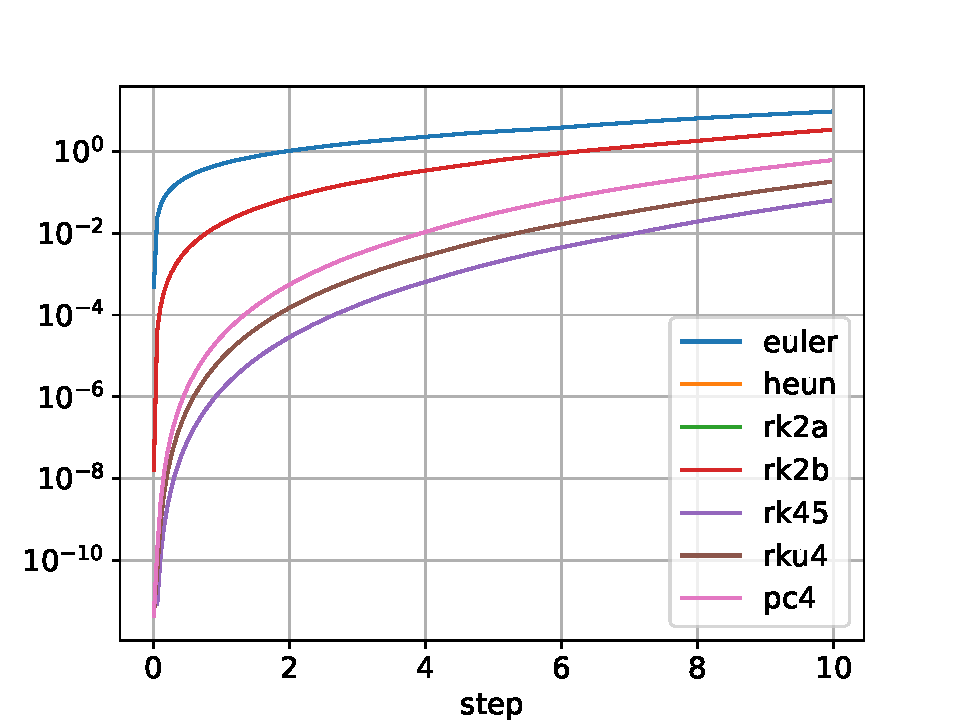
\includegraphics[width=\linewidth]{precision.pdf}
		\caption{Največji odmik od teoretične rešitve na območju $t \in [0, 500]$}
    \end{subfigure}
    \hfill
    \begin{subfigure}{0.49\textwidth}
        \centering
		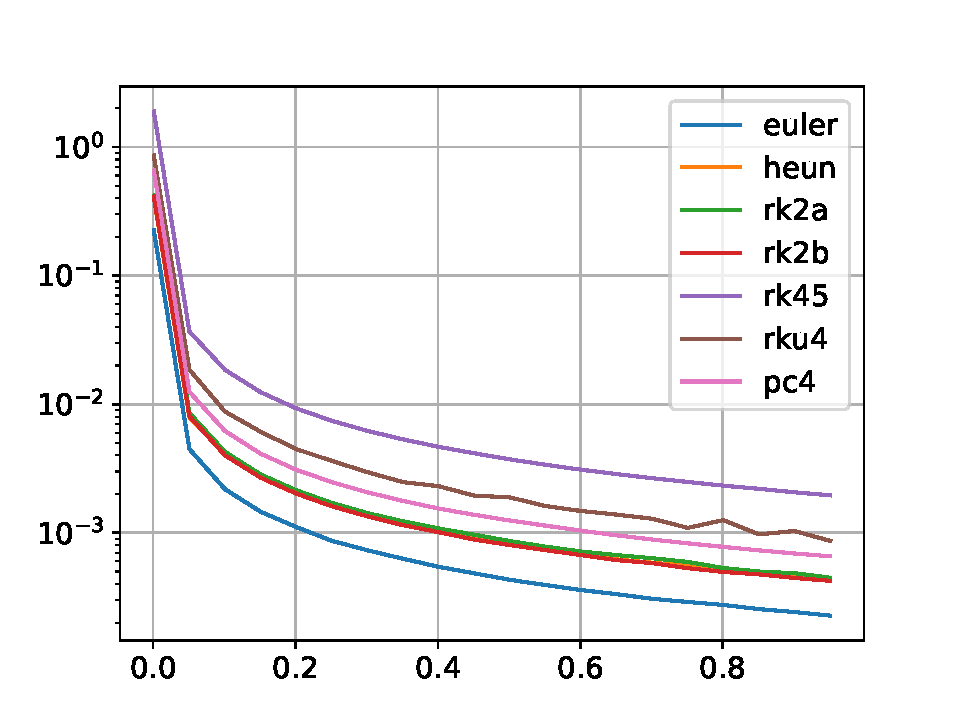
\includegraphics[width=\linewidth]{time.pdf}
		\caption{Časovna zahtevnost metod}
    \end{subfigure}
	\caption{Odvisnosti od velikosti koraka}
\end{figure}
Grafa sta pri majhnih vrednostih precej dolgočasna, saj kot pričakovano z velikostjo koraka natančnost in časovna zahtevnost padata. Pri vrednostih blizu ničle pa ravno obratno.
Pobližje poglejmo še obnašanje metod za našo izbiro. Opazimo, da imata ,etodi RK2a in RK2b enako natačnost in približno enako časovno zahtevnost. Kar je tudi pričakovano, saj sta obe metodi drugega reda.
Eulerjeva metoda je sicer najhitrejša, a je njena natančnost precej slabša od ostalih. 
Najbolj natančni pa sta metodi RK4 in RK45. Metoda RK4 je hitrostno precej bolj primerljiva z ostalimi. S čemer lahko tudi pojasnimo njeno popularnost.
\\
Omembe vredna je tudi odvisnost natančnosti pri višjih vrednostih koraka, ki pa za nas ni relevantna se pa v njej pojavijo določene anomalije, ki so brez podrobnega znanja metod težko razložljive.
\begin{figure}[H]
    \centering
    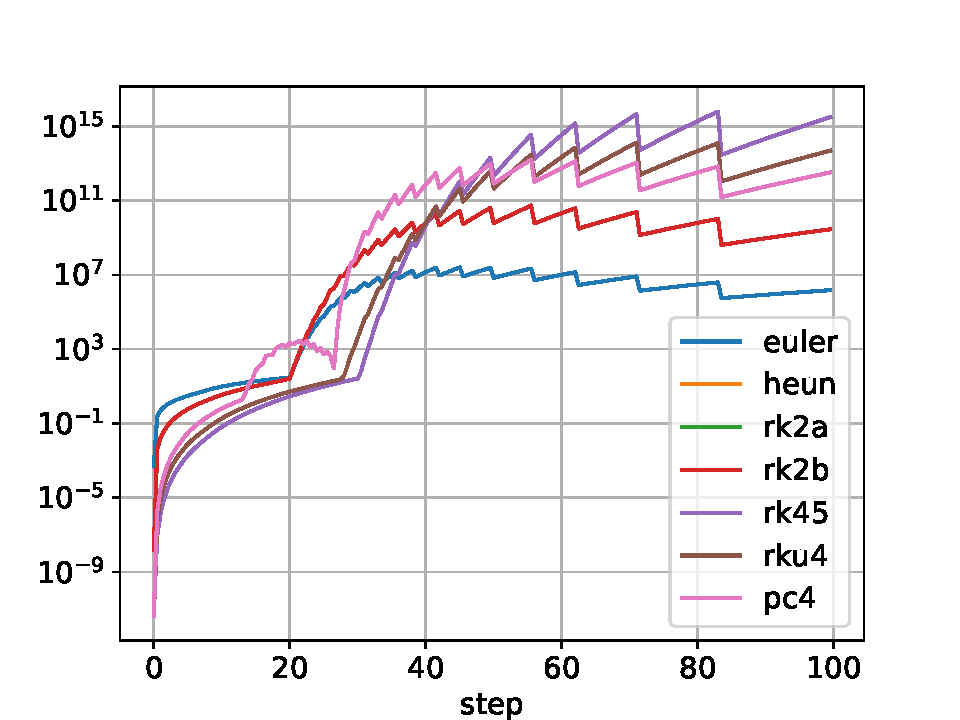
\includegraphics[width=0.5\textwidth]{precisionbig.pdf}
	\caption{Največji odmik od teoretične funkcija za večje vrednosti}

    \label{fig:sample_image}
\end{figure}
\subsection{Družine rešitev}
S prejšnjim raziskovanjem se tako odločimo, da bomo pri iskanju družine rešitev uporabili metodo Runge-Kutta 4.\ reda s korakom $h=0.1$. Za vizualizacijo rešitev pri različnih vrednosti parametra $k$ uporabimo barvo kot dodano dimenzijo, ki v našem primeru predstavlja temperaturo.

\begin{figure}[H]
    \centering
    \begin{subfigure}{0.49\textwidth}
        \centering
        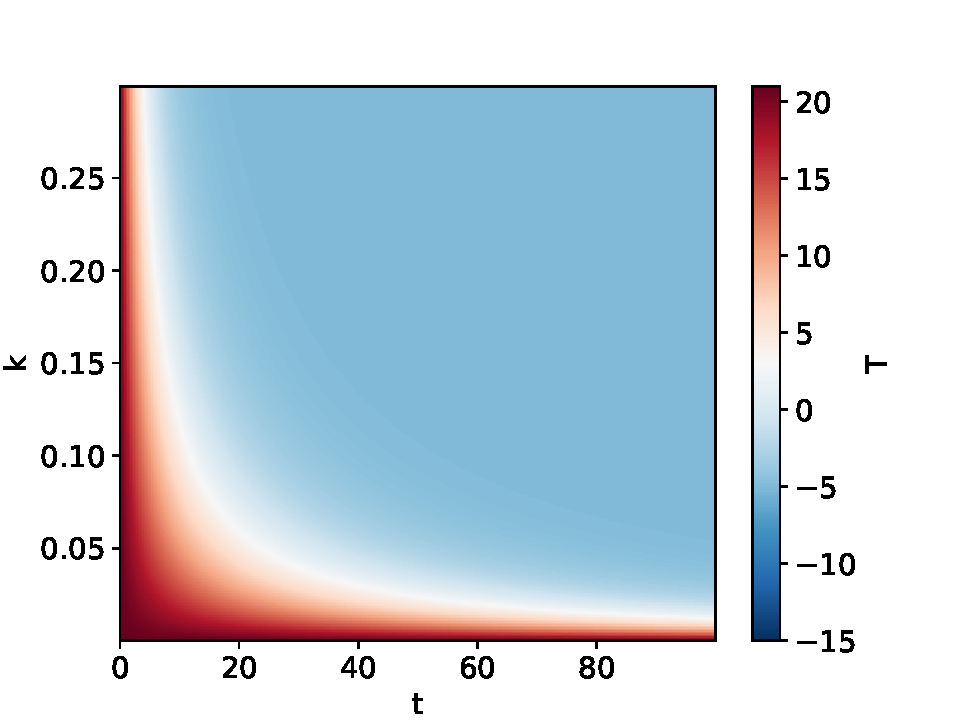
\includegraphics[width=\linewidth]{family21.00.pdf}
		\caption{Pri začetni temperaturi $T_0=21$}
        \label{fig:image1}
    \end{subfigure}
    \hfill
    \begin{subfigure}{0.49\textwidth}
        \centering
		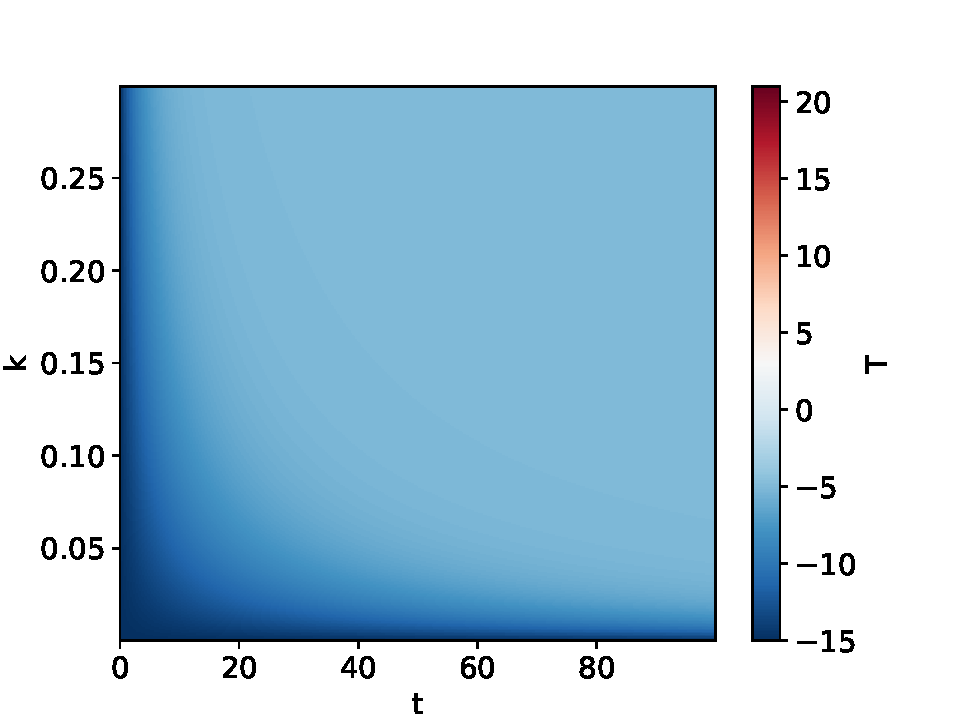
\includegraphics[width=\linewidth]{family-15.00.pdf}
		\caption{Pri začetni temperaturi $T_0=-15$}
        \label{fig:image2}
    \end{subfigure}
	\caption{Vizualizacija rešitev pri različnih vrednostih parametra $k$}
\end{figure}
\subsection{Dodatna naloga}
Za dodatno nalogo pa naši imaginarni sobi dodamo še sonce, ki jo periodično ogreva. Velikost koraka in metodo smo ohranili kot pri računanju brez sonca. Za računanje uporabimo podano diferencialno enačbo $\frac{dT}{dt}=-k(T-T_{zun}) + A \sin{\left(\frac{2\pi}{24}(t - \delta)\right)}$. V prvem paru grafov je fiksna vrednost $A=1$ in dodamo za spremenljivko parameter $k$. V drugem paru obrnemo vloge in fiksiramo $k=0.1$. Glede na enačbo in tudi rezultat opazimo, da prvi člen diferencialne postaja vedno manjši in se nato temperatura `ustali` na sinusnem valu. Če bi želeli posebej natančno določiti maksimalne temperature in trenutke, ko nastopijo pa bi verjetno  našo metodo morali nadomestiti s kakšno drugo, ki prilagaja korak glede na pogoje v danem trenutku. Primera takih metod sta RKF45 in Dormand-Prince.

\begin{figure}[H]
    \centering
    \begin{subfigure}{0.49\textwidth}
        \centering
        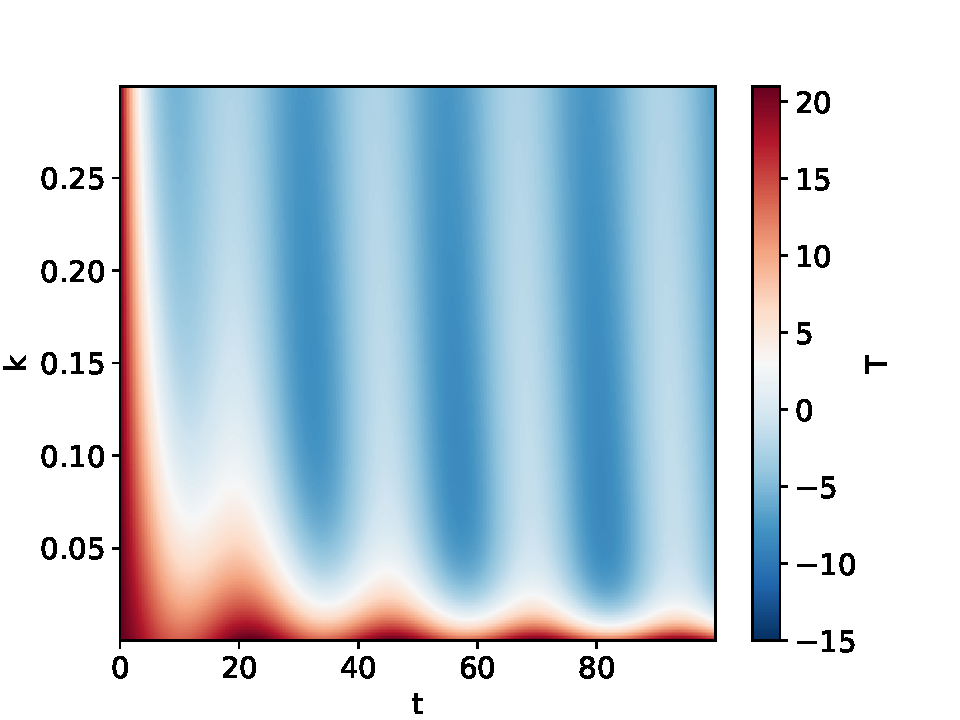
\includegraphics[width=\linewidth]{family21.01.pdf}
		\caption{Pri začetni temperaturi $T_0=21$}
        \label{fig:image1}
    \end{subfigure}
    \hfill
    \begin{subfigure}{0.49\textwidth}
        \centering
		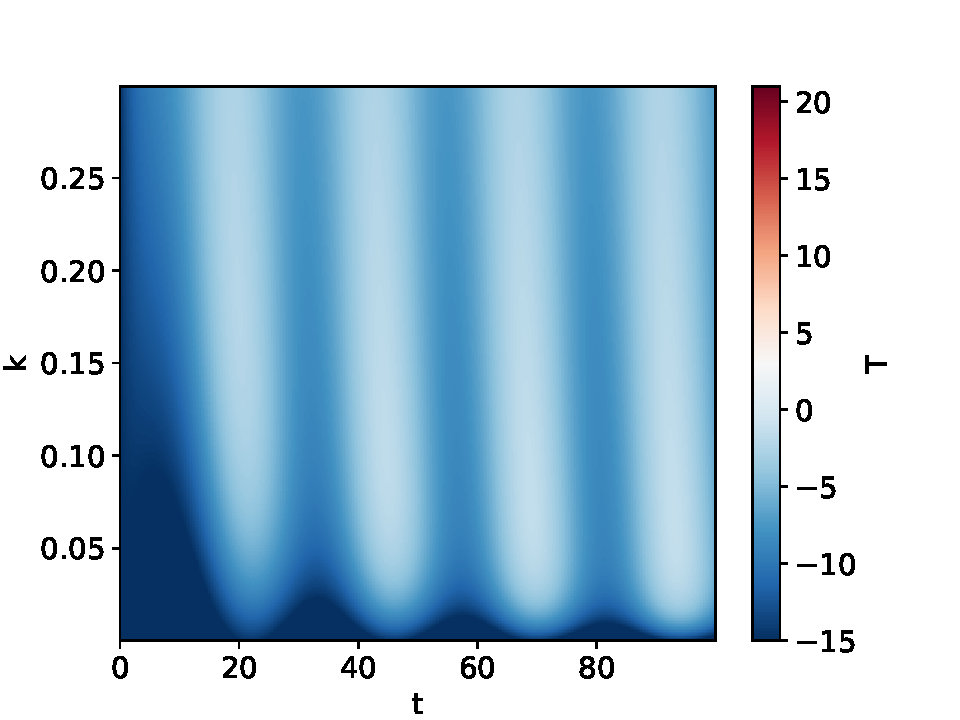
\includegraphics[width=\linewidth]{family-15.01.pdf}
		\caption{Pri začetni temperaturi $T_0=-15$}
        \label{fig:image2}
    \end{subfigure}
	\caption{Vizualizacija rešitev pri različnih vrednostih parametra $k$}
\end{figure}

\begin{figure}[H]
    \centering
    \begin{subfigure}{0.49\textwidth}
        \centering
        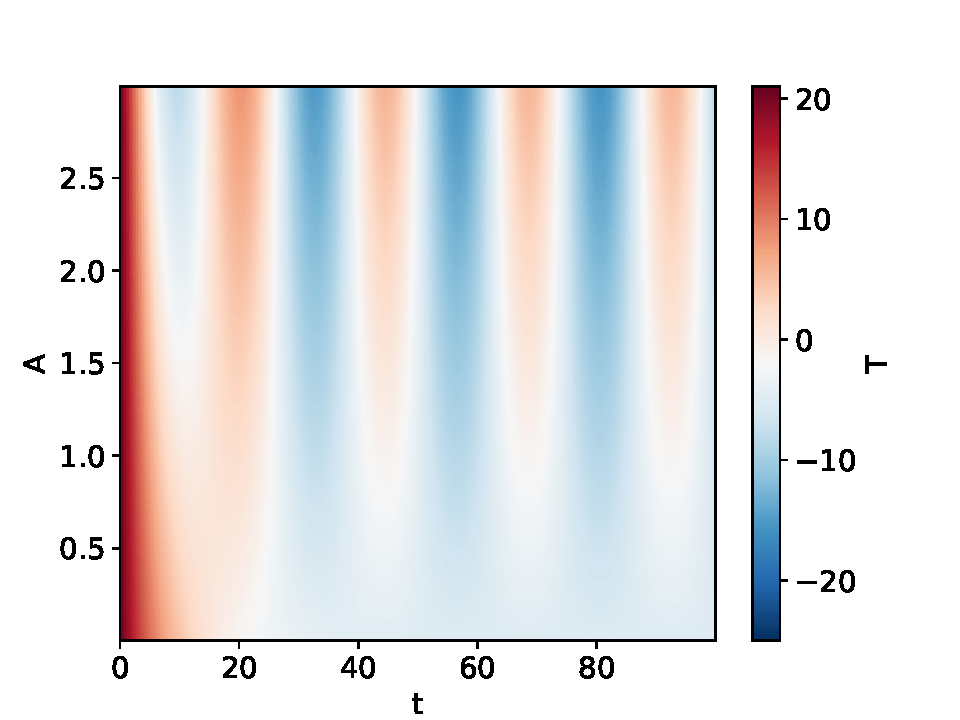
\includegraphics[width=\linewidth]{family21.02.pdf}
		\caption{Pri začetni temperaturi $T_0=21$}
        \label{fig:image1}
    \end{subfigure}
    \hfill
    \begin{subfigure}{0.49\textwidth}
        \centering
		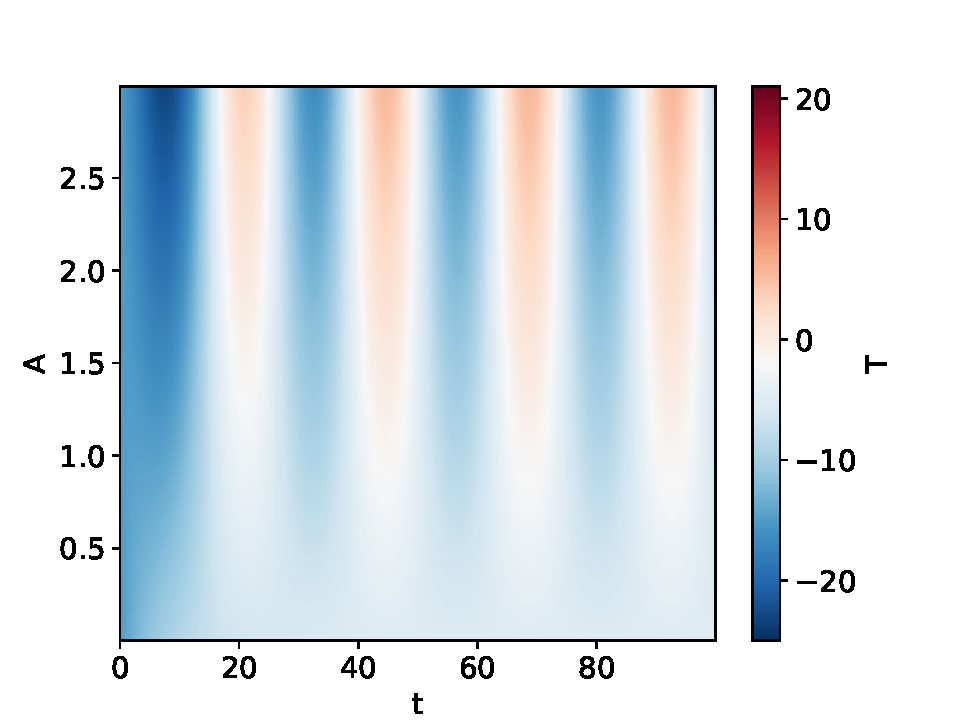
\includegraphics[width=\linewidth]{family-15.02.pdf}
		\caption{Pri začetni temperaturi $T_0=-15$}
        \label{fig:image2}
    \end{subfigure}
	\caption{Vizualizacija rešitev pri različnih vrednostih parametra $A$}
\end{figure}
\newpage
\section{Zaključek}
V nalogi smo se spoznali z različnimi metodami numerične integracije in njihovim obnašanjem. Naloga mi je bila do zdaj najmanj zanimiva. Verjetno zaradi tega, ker je problem zelo pogost in sem se z njim srečal že velikokrat. Je bilo pa poučno izvedeti nekaj več o Runge-Kutta metodah, saj sem jih prej pogosto le uporabljal. Za konec pa dodajam še graf o hitrosti govorjenja in podajanja informacij v različnih jezikih.
\begin{figure}[H]
    \centering
    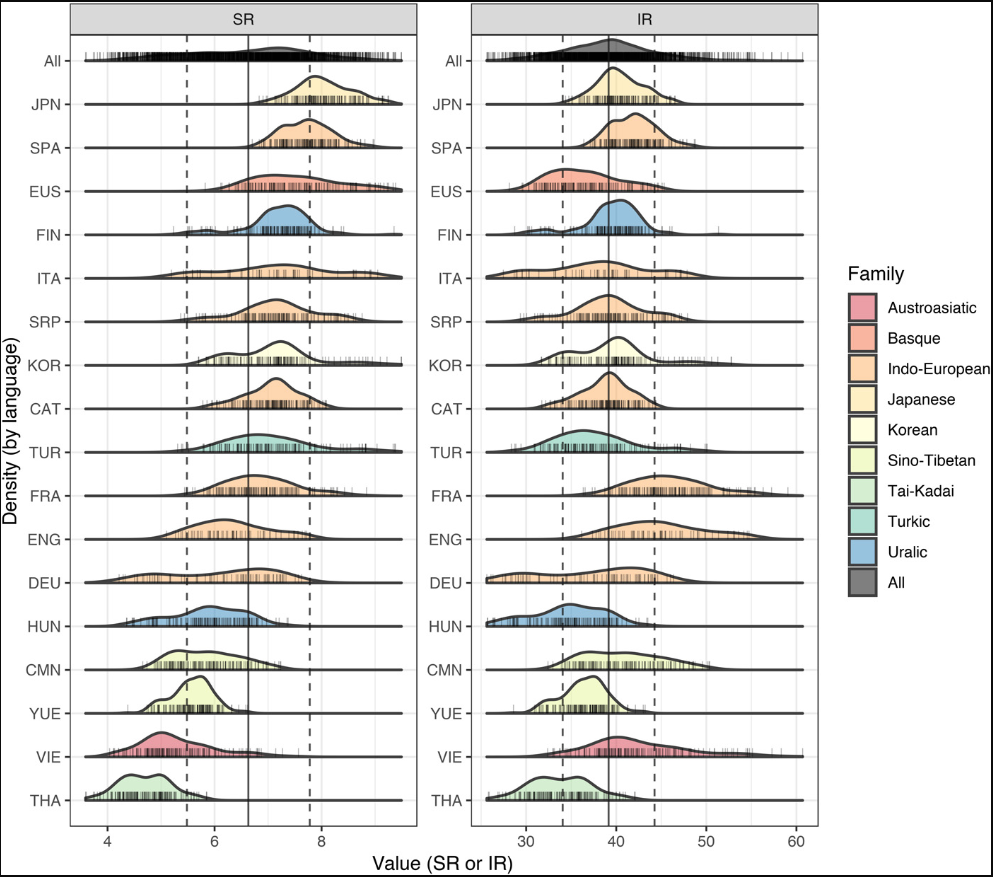
\includegraphics[width=0.8\textwidth]{languages.png}
	\caption{Vir: ``Different languages, similar encoding efficiency: Comparable information rates across the human communicative niche`` by Cristophe Coupè, Yoon Mi Oh, Dan Dediu and Francois Pellegrino, Science Advances(2019)}
    \label{fig:image_label}
\end{figure}
\end{document}
